%
% $RCSfile: brain_regions.tex,v $
%
% Copyright (C) 2002-2008. Christian Heller.
%
% Permission is granted to copy, distribute and/or modify this document
% under the terms of the GNU Free Documentation License, Version 1.1 or
% any later version published by the Free Software Foundation; with no
% Invariant Sections, with no Front-Cover Texts and with no Back-Cover
% Texts. A copy of the license is included in the section entitled
% "GNU Free Documentation License".
%
% http://www.cybop.net
% - Cybernetics Oriented Programming -
%
% http://www.resmedicinae.org
% - Information in Medicine -
%
% Version: $Revision: 1.1 $ $Date: 2008-08-19 20:41:05 $ $Author: christian $
% Authors: Christian Heller <christian.heller@tuxtax.de>
%

\subsection{Brain Regions}
\label{brain_regions_heading}
\index{Brain Regions}
\index{Central Nervous System}
\index{CNS}
\index{Peripheral Nervous System}
\index{PNS}

\emph{Neurology} as branch of \emph{Medicine} deals with the
\emph{Central Nervous System} (CNS) and \emph{Peripheral Nervous System} (PNS)
of human beings. These can be further divided as shown in figure
\ref{nervoussystem_figure}.

\begin{figure}[ht]
    \begin{center}
        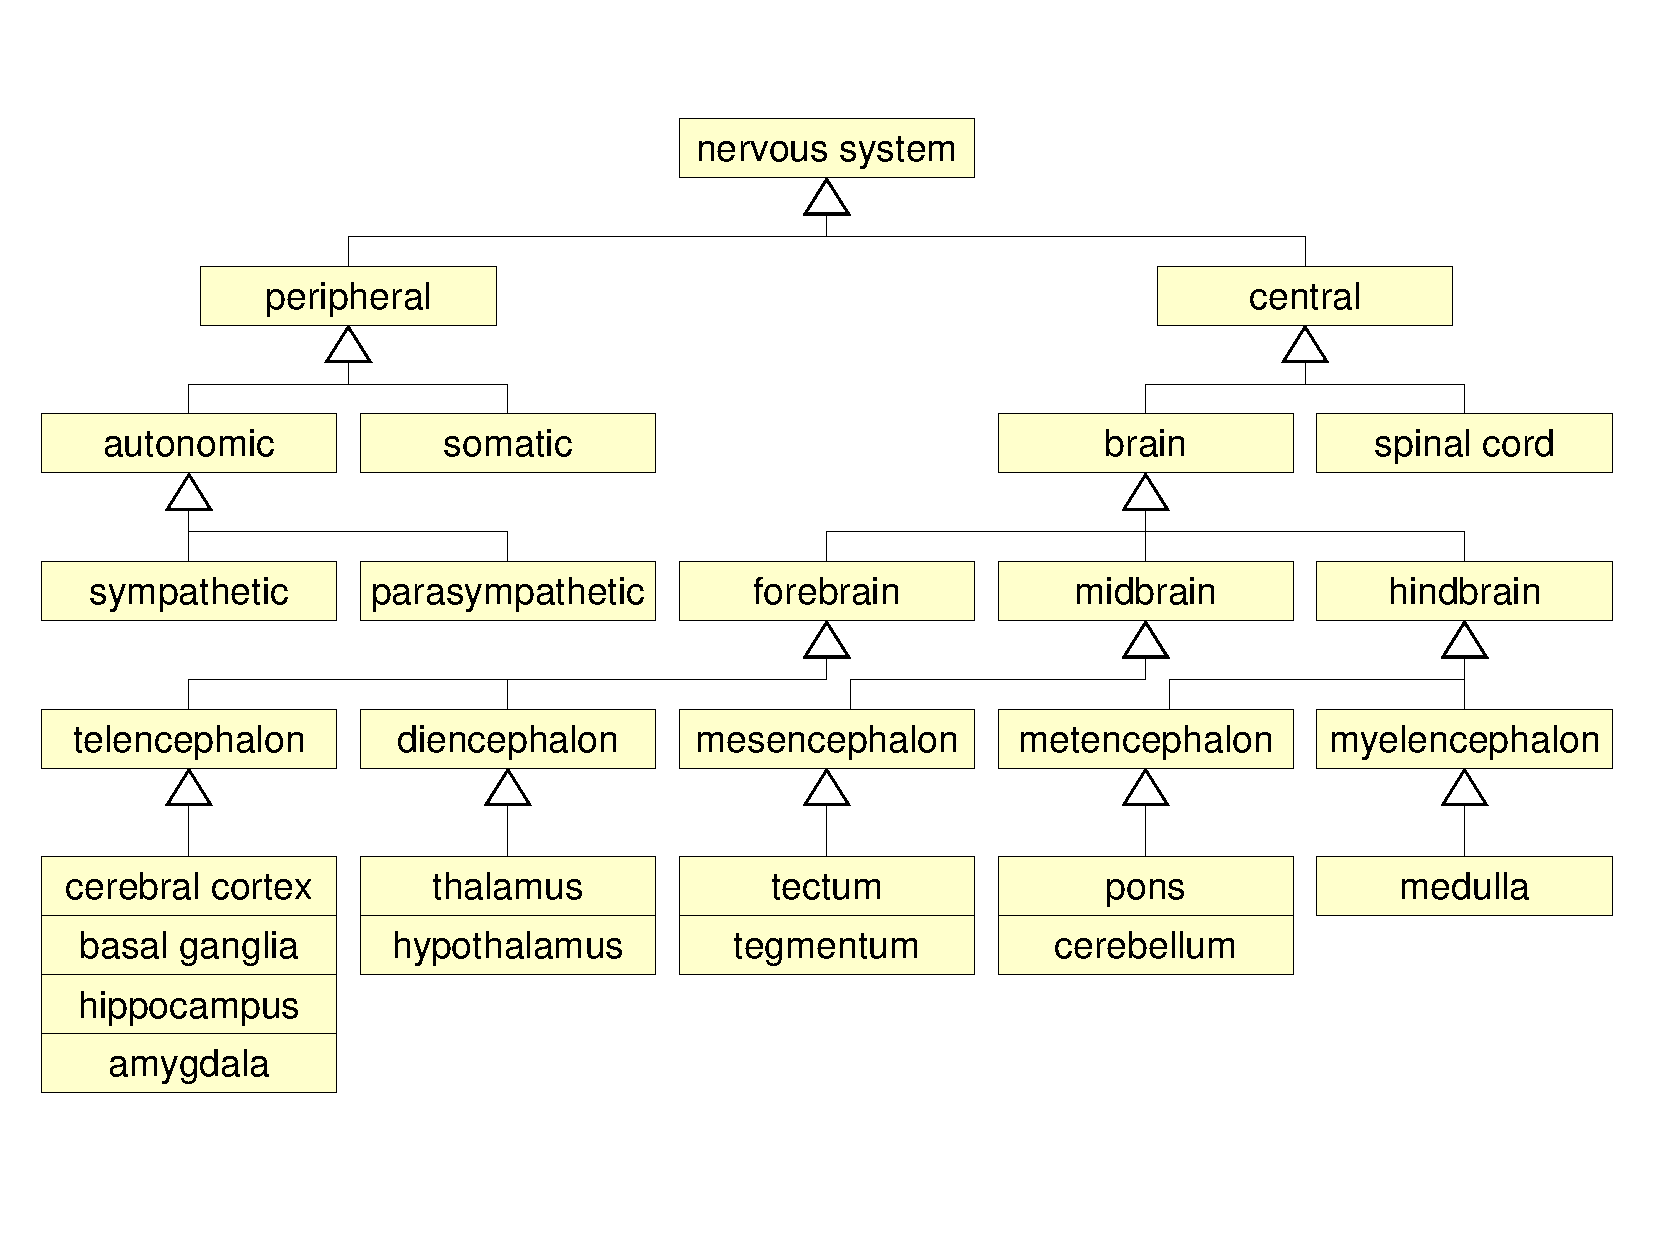
\includegraphics[scale=0.3,angle=-90]{graphic/nervoussystem.pdf}
        \caption{Divisions of the Nervous System \cite{adventuresinneuroanatomy}}
        \label{nervoussystem_figure}
    \end{center}
\end{figure}

Not all parts of this systematics shall be explained here; more details can be
found at \cite{pschyrembel}. Chapter \ref{state_and_logic_heading} will make
some remarks on the PNS, whose \emph{Neurons} (nerve cells) can be functionally
divided into \emph{sensory} (\emph{afferent}) and \emph{motor}
(\emph{efferent}) ones. The functions of some brain structures, as part of the
CNS, are described in table \ref{brainstructures_table}. At the same time, this
table (where \emph{n/a} means \emph{not applicable}) tries to give possible
analogies to a standard computer system, whereby hardware as well as software
are considered.

\begin{table}[ht]
    \begin{center}
        \begin{footnotesize}
        \begin{tabular}{| p{25mm} | p{50mm} | p{30mm} |}
            \hline
            \textbf{Brain Structure} & \textbf{Function} & \textbf{Computer Analogon}\\
            \hline
            Cerebral Cortex
            & Thought, Voluntary Movement, Language, Reasoning, Perception
            & Application/ Domain Knowledge\\
            \hline
            Cerebellum
            & Movement, Balance, Posture
            & n/a (only in Robots)\\
            \hline
            Brain Stem %(medulla, pons, tectum, tegmentum)
            & Breathing, Heart Rate, Blood Pressure
            & Timer, Power Supply\\
            \hline
            Hypothalamus
            & Body Temperature, Hunger, Thirst, Emotions, Circadian Rhythms
            & Self-observing Sensors (Battery-/ CPU Status)\\
            \hline
            Thalamus
            & Sensory Processing, Information Forwarding, Movement
            %(cerebral cortex [forwards information] to other brain areas and spinal cord)
            & Event Mechanism, Signal Loop, IRQ Handler\\
            \hline
            Limbic System %(amygdala, hippocampus)
            & Emotions
            & Signal Priorities\\
            \hline
            Hippocampus
            & Learning, Memory
            & Knowledge Storage, RAM\\
            \hline
            Basal Ganglia %(globus pallidus, caudate nucleus,
            %subthalamic nucleus, putamen, substantia nigra)
            & Movement
            & n/a (only in Robots)\\
            \hline
            Midbrain %(superior/ inferior colliculi, red nucleus)
            & Vision, Audition, Eye- and Body Movement
            & I/O Device Drivers, Translation\\
            \hline
        \end{tabular}
        \end{footnotesize}
        \caption{Brain Structures in Analogy to a Computer \cite{adventuresinneuroanatomy}}
        \label{brainstructures_table}
    \end{center}
\end{table}

Of course, the analogies do not match exactly. Also, there are many functions
-- like \emph{Thought} or \emph{Emotions} -- that a computer cannot perform.
The important thing to notice, however, is that there are brain regions mainly
\emph{storing} (Hippocampus) and \emph{applying} knowledge (Cerebral Cortex) and
others \emph{coordinating} the input/ output (i/o) of that knowledge (Midbrain,
Basal Ganglia) in form of simplified information, through sensoric/ motoric
organs of the human body.

That is, what philosophy calls \emph{Mind} (section \ref{mind_and_body_heading})
is the \emph{Knowledge} that is anatomically-physically mainly situated in the
\emph{Hippocampus} and \emph{Cerebral Cortex}. And again, i/o control does not
only rely on hardware devices but also on the corresponding driver software and
signalling mechanism. To say it differently: The software that contains
application/ domain knowledge is to be treated \emph{separately} from system
control software.
